    \documentclass[13,twocolumn,letterpaper]{article}
    \usepackage[spanish,english]{babel}
    \usepackage[utf8x]{inputenc}
    \usepackage[T1]{fontenc}
    \usepackage[a4paper,top=3cm,bottom=2cm,left=3cm,right=3cm,marginparwidth=1.75cm]{geometry}
    \usepackage{amsmath}
    \usepackage{graphicx}
    \usepackage[colorinlistoftodos]{todonotes}
    \usepackage[colorlinks=true, allcolors=blue]{hyperref}
    \usepackage{float}
    
    \title{
    		%\vspace{-1in} 	
    		\usefont{OT1}{bch}{b}{n}
    		\normalfont \normalsize \textsc{INSTITUTO POLITÉCNICO NACIONAL \\ 
    		ESCUELA SUPERIOR DE FISICA Y MATEMATICAS \\
    		ACADEMIA DE FÍSICA EXPERIMENTAL} \\ 
    	 FÍSICA IV: LABORATORIO DE ÓPTICA. \\[10pt]
    		\huge Práctica III: \\
    	Determinación de la Longitud Focal de Lentes Delgadas \\
    }
    
    \usepackage{authblk}
    \author[0]{Alumno: Flores Rodriguez Jaziel David \\
    Boleta: 2014030429 \\
    Profesor: Dr. Janos Zsargo\\
    Grupo: 4FV2-B \\
            }
    \begin{document}
    \maketitle
    
    \selectlanguage{spanish}
    
    \section*{Resumen}
    
    En esta práctica se realizaron dos experimentos, haciendo uso de las ecuaciones de Gauss y de Newton, para estudiar la formación de imágenes usando lentes delgadas. 
    En el primer experimento, se observó la formación de imágenes a través de una lente
    delgada positiva, se fue variando la distancia entre la lente y el objeto usando
    distintos múltiplos de la distancia focal y se midió la longitud de cada una de las
    imágenes. \\
    En el segundo experimento se utilizaron dos lentes; la primera lente negativa, con la
    que formaron imágenes virtuales y la segunda lente positiva con la que “se convertían”
    las imágenes virtuales formadas con la lente negativa en imágenes reales, ello
    con el fin de repetir procedimiento de variar las distancias y medir las imágenes
    formadas
    
    
    \section*{Introducción}
    
    \textbf{Lentes}: Una lente es un sistema óptico limitado por dos o más superficies
    refringentes que tienen un eje común. Si la lente sólo tiene dos superficies,
    se denomina lente sencilla; si tiene más de dos, se trata de una lente
    compuesta.
    Todas las lentes de alta calidad son lentes compuestas; es decir, están
    formadas por un cierto número de lentes sencillas que tienen un eje
    común. \\
    \textbf{Lentes delgadas}:
    Puede considerarse que toda la desviación producida en
    un rayo cualquiera al atravesar una lente delgada se verifica en un plano
    que pasa por el centro de la lente. Esto es, los planos principales objeto
    e imagen de una lente delgada coinciden; por tanto, coinciden también
    los puntos principales objeto e imagen, que a su vez lo hacen con el centro
    de la lente. Según esto la distancia focal de una lente delgada es
    simplemente la distancia desde el centro de la lente a cada foco.
    En general, las lentes delgadas pueden considerarse como líneas.
    
    
    \section*{Lentes Delgadas} 
    
    
    Existen muchos ejemplos comunes de la refracción de la luz por una lente. Las lentes de nuestros ojos  enfocan  la  luz  de  la  retina,  mientras  que  las  lentes  correctoras  de  los  anteojos  o  lentes  de contacto compensan  las deficiencias en  nuestra  visión. La  lente de múltiples elementos de una cámara enfoca la luz en la película. En la mayoría de las situaciones de refracción existe más de una superficie refringente.  Esto es  cierto  incluso para una  lente de contacto, donde  la  luz pasa primero  del  aire  al  vidrio  y  después  del  vidrio  a  nuestro  ojo.  Aquí  sólo  se  considera  el  caso especial de una lente delgada; es decir, el espesor de la lente es pequeño en comparación con la distancia sodel objeto, la distancia side la imagen, o los radios de curvatura r1y r2de cualquiera de las dos superficies refringentes. En una lente, estas cantidades se relacionan según: 
    
    \[ \frac{1}{s_{o}} +  \frac{1}{s_{i}} = \frac{1}{f} \]
    
    Donde la distancia focal fde la lente está dada por:
    
    \[ \frac{1}{f} = (n-1)(\[ \frac{1}{r_{1}} +  \frac{1}{r_2} )  \]
    
    Las  ecuaciones  1  y  2  son  aproximaciones  que  se  cumplen  sólo  para  lentes  delgadas  y  rayos paraxiales.
    
    
    \section*{Convenciones de signos}
   Los radios de curvatura $r_{1}$ relativos a la primera superficie sobre la que incide la luz) y $r_{2}$
(relativo a  la  segunda  superficie  sobre  la  que  incide  la  luz)  son  positivos  si  los  centros  de  curvatura correspondientes  están  en  el  lado V. \\En  la  parte  a  de  la  figura  1,  el  centro  de  curvatura $C_{1}$
se encuentra en el lado R, así que $r_{1}$
es positivo, mientras que $C_{2}$
se encuentra en el lado V, por lo cual $r_{2}$ es negativo.  \\
Al observar la ecuación 1 esta demuestra que, cuando $r_{1}$>0 y $r_{2}$<0, la distancia focal f
siempre es positiva. Tal lente se llama lente convergente; una lente que es más gruesa en el centro que en los extremos, cuando está inmersa en un medio de índice de refracción menor que el de la lente, es siempre una lente convergente. 
    
    \begin{figure}[h!]
      \centering
      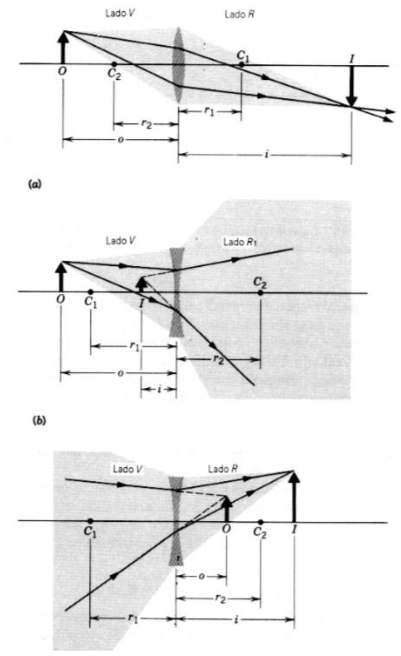
\includegraphics[width=0.4\textwidth]{PRIMERA.png}
      \caption{\\
      (a) Se forma una imagen real, invertida mediante una lente convergente. Tal lente tiene una distancia focal positiva  y  es  más  gruesa  en  el  centro  que  en  los extremos. \\ \\
      (b)  Se  forma  una  imagen  virtual,  directa  mediante una  lente  divergente.  Tal  lente  tiene  una  distancia focal negativa y es más delgada en el centro que en los extremos.\\ \\
      (c)  La  luz  converge  de  un  objeto  virtual  en O.  Se forma  una  imagen  real,  directa  en Imediante  esta lente divergente.}
    \end{figure}
    
    
  
    \section*{Desarrollo Experimental}
    
        \subsection*{Experimento 1: Método Directo} Con la ayuda de un láser y una óptica de expansión del rayo, se hizo incidir el haz sobre la lentey  se  desplazó  una  pantalla  hasta  que  se  obtuvo  un  punto  nítido  sobre  esta.  Asegurándonos  de haber localizado el punto focal y se determinó dicha distancia.Se utilizaron dos lentes una con una distancia focal del fabricante igual a 200mm y otra de 100mm.
        \\ \\
        Posteriormente se realizaron
        las
        mismas
        mediciones, pero se giraron
        las
        lentes, observándose las
        otras
        carasa la incidencia del rayo láser.

    \begin{figure}[H]
      \centering
      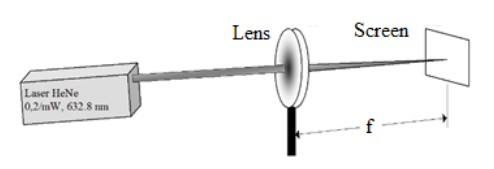
\includegraphics[width=0.4\textwidth]{Segunda.png}
      \caption{Arreglo experimental.}
      
    \end{figure}
    
    
    
        \subsection*{Experimento 2: Método de autocolimación}
        
        
        Se tenía un arreglo como en la figura 3. Aquí variamos la distancia entre la lente y la rendija hasta que obtuvimos una imagen nítida del objeto dela rendija en la misma rendija, así garantizamos que  la  distancia  entre  la  lente  y  la  rendija  es  igual  a  la  distancia  focal.  Se  realizó  la  misma medición de la distancia focal girando la lente para observar la otra cara a la incidencia. Esto con dos lentes distintas, una con distancia focal del fabricante igual a 200mm y 100mm.

    \begin{figure}[H]
      \centering
      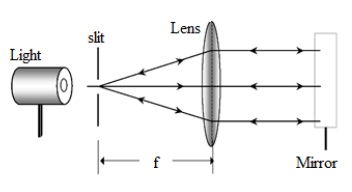
\includegraphics[width=0.4\textwidth]{Tercera.png}
      \caption{Arreglo experimental.}
      
    \end{figure}
    
       \subsection*{Experimento 3: Método de doble desplazamiento
       }
        
        Se  tenía  un  arreglo
        como  el  que  se  muestra  en  la  figura  4. Se  movió  la  lente  hasta  que  en  la posición  1  se  encontró  la  imagen  nítida  de  la  rendija  en  la  pantalla  y  se  midió  esa  distancia, después se deslizó la lente hasta la posición 2 en donde se encontró también la imagen nítida de la rendija en la pantalla e igualmente se midió esa distanciaque denotaremos por d, a la distancia que hay entre la rendija y la pantalla la denotaremos por D. Se realizaron estas mediciones para una lente de distancia focal del fabricante iguala 100mm y otra de 200mm.
        
    \begin{figure}[H]
      \centering
      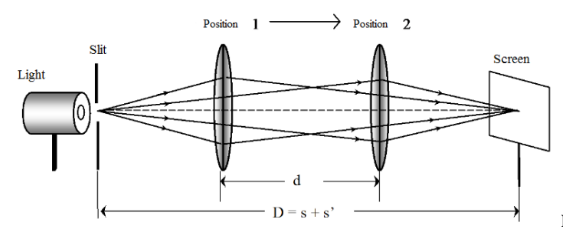
\includegraphics[width=0.5\textwidth]{Cuarta.png}
      \caption{Arreglo experimental.}
      
    \end{figure}
    
    \section*{Resultados} 
    
     \subsection*{Experimento 1: Método Directo}
     
Para  la  primera  lente  que  utilizamos  se  obtuvieron  las  siguientes  medicionespara  la  distancia focal. 

    \begin{table}[h]
        \centering
        \begin{tabular}{|| c | c || }
                \hline
                \hline
\textbf{Sin Girar} & \textbf{ Girando}\\ \hline
100 mm  & 103 mm \\ \hline
\hline
   \end{tabular}
    \caption{Primer Lente}
    \end{table}
    
Sabiendo que la distancia focal del fabricante es igual a 100 mm es posible calcular el error para
ambos casos, entonces para el caso sin girar la lente se tiene

\[ \epsilon =  \left | \frac{f_{t} - f_{m}}{ f_{t} }\right | \times
100=  \left | \frac{100 - 100}
{100 }\right | \times 
100 = 0\%
\]

Cuando se gira la lente se tiene:

\[ \epsilon =  \left | \frac{f_{t} - f_{m}}{ f_{t} }\right | \times
100=  \left | \frac{100 - 103}
{100 }\right | \times 
100 = 3\%
\]

Ahora para la segunda lente se obtuvieron las siguientes mediciones.

\begin{table}[h]
        \centering
        \begin{tabular}{|| c | c || }
                \hline
                \hline
\textbf{Sin Girar} & \textbf{ Girando}\\ \hline
205 mm  & 208 mm \\ \hline
\hline
   \end{tabular}
    \caption{Segunda Lente}
    \end{table}

Igualmente sabiendo que la distancia focal del fabricante es igual a 200 mm es posible calcular
el error en nuestras mediciones, entonces sin girar la lente se tiene que 

\[ \epsilon =  \left | \frac{f_{t} - f_{m}}{ f_{t} }\right | \times
100=  \left | \frac{200 - 205}
{200 }\right | \times 
100 =  2.5\%
\]

Al girar la lente se tiene que 

\[ \epsilon =  \left | \frac{f_{t} - f_{m}}{ f_{t} }\right | \times
100=  \left | \frac{200 - 208}
{200 }\right | \times 
100 =  4\%
\]  
    
 \subsection*{Experimento 2: 
 Método de autocolimación
 }
 Para la primera lente se obtuvieron las siguientes mediciones:
 
 \begin{table}[h]
        \centering
        \begin{tabular}{|| c | c || }
                \hline
                \hline
\textbf{Sin Girar} & \textbf{ Girando}\\ \hline
96 mm  & 97 mm \\ \hline
\hline
   \end{tabular}
    \caption{Primer Lente}
    \end{table}
 
 Conociendo que la distancia focal del fabricante es igual a 100 mm es posible calcular el error,
entonces para la lente se girar se tiene que:

\[ \epsilon =  \left | \frac{f_{t} - f_{m}}{ f_{t} }\right | \times
100=  \left | \frac{100 - 96}
{100 }\right | \times 
100 =  4\%
\]  

Al girar la lente se obtuvo que 

\[ \epsilon =  \left | \frac{f_{t} - f_{m}}{ f_{t} }\right | \times
100=  \left | \frac{100 - 97}
{100 }\right | \times 
100 =  3\%
\]  

Para la segunda lente se obtuvo que: 

 \begin{table}[h]
        \centering
        \begin{tabular}{|| c | c || }
                \hline
                \hline
\textbf{Sin Girar} & \textbf{ Girando}\\ \hline
200 mm  &  199  mm \\ \hline
\hline
   \end{tabular}
    \caption{Primer Lente}
    \end{table}

Igualmente teniendo que la distancia focal del fabricante es igual a 200 mm fue posible obtener
el error, para la lente sin girar se tiene que 

\[ \epsilon =  \left | \frac{f_{t} - f_{m}}{ f_{t} }\right | \times
100=  \left | \frac{200 - 200}
{200 }\right | \times 
100 =  0\%
\]  

Girando la lente se obtiene que 

\[ \epsilon =  \left | \frac{f_{t} - f_{m}}{ f_{t} }\right | \times
100=  \left | \frac{200 - 199}
{200 }\right | \times 
100 =  0.5\%
\]  

 \subsection*{Experimento 3: 
 Método de doble desplazamiento
 }
En este método para obtener la distancia focal se utilizará la fórmula:

\[ f =    \frac{ {D}^2 -  {d}^2}{ 4D }
\]  

Entonces para la primera lente se obtuvieron las siguientes mediciones

\begin{table}[H]
        \centering
        \begin{tabular}{|| c | c || }
                \hline
                \hline
\textbf{D} & \textbf{ d }\\ \hline
700 mm  &  463  mm \\ \hline
\hline
   \end{tabular}
    \caption{Primer Lente}
\end{table}
    
Utilizando la fórmula obtenemos que la distancia focal es igual a 98.4396 mm y como la distancia focal del fabricante es igual a 100 mm se puede calcular el error: 

\[ \epsilon =  \left | \frac{f_{t} - f_{m}}{ f_{t} }\right | \times
100=  \left | \frac{ 100 − 98.4396}
{100 }\right | \times 
100 =  1.56\%
\]  

Para la segunda lente se obtuvieron las siguientes mediciones: 

\begin{table}[H]
        \centering
        \begin{tabular}{|| c | c || }
                \hline
                \hline
\textbf{D} & \textbf{ d }\\ \hline
850 mm  &  211  mm \\ \hline
\hline
   \end{tabular}
    \caption{Segunda Lente}
\end{table}


Calculando la distancia focal con la fórmula dada anteriormente tenemos que esta es igual a 199.4
mm, la distancia focal del fabricante es igual a 200 mm, así calculando el error se obtiene 

\[ \epsilon =  \left | \frac{f_{t} - f_{m}}{ f_{t} }\right | \times
100=  \left | \frac{ 200 − 199.4
}
{200 }\right | \times 
100 =  0.3\%
\]  


 \subsection*{Conclusiones}

Es posible observar en los resultados que el error en nuestras mediciones es muy pequeño,
concluyendo que los distintos métodos para medir distancias focales utilizados en esta práctica
son fiables para determinar dicho dato en una lente.


\medskip
\medskip
\medskip
\medskip
\medskip
\medskip
\medskip
\medskip
\medskip\medskip
\medskip
\medskip\medskip
\medskip
\medskip
\medskip
\medskip
\medskip\medskip
\medskip
\medskip\medskip
\medskip
\medskip
\medskip\medskip
\medskip
\medskip\medskip
\medskip
\medskip

    \begin{thebibliography}{9}
    \bibitem{a_reference} 
    Física Vol. 2, versión ampliada, cuarta edición en español, capítulo 44, pp. 377-379.

    \bibitem{other_ref}
   https://es.wikipedia.org/wiki/Distancia\_focal
    
   
    
    \end{thebibliography}
    
    \end{document}